\section{Documentation on Army Hierarchy}

\subsection{Overview}

This version of the code constructs a hierarchical graph based on a custom ranking system, in this case, the U.S. Air Force rank hierarchy. Each node in the graph corresponds to a rank, represented not by its name but by a symbolic representation (e.g., stars for generals, different symbols for enlisted ranks).
The logic is similar to previous versions that used letters:

\begin{itemize}
\item     Each character in the input string (A, B, C, ..., up to V) maps to a specific rank level.
    
\item     The hierarchy is top-down, with A representing the highest rank (General of the Air Force) and subsequent letters representing progressively lower ranks.
    
\item     Sibling nodes (nodes of the same level under the same parent) are connected horizontally to show their relationship.
    
\item    The \# character breaks the sibling chain, ensuring that a node following \# will not link to its previous sibling.
\end{itemize}

\subsection{Key Concepts}

\begin{enumerate}
    \item \textbf{Hierarchy by Rank:} 
    \begin{itemize}
        \item  The code uses a predefined list of U.S. Air Force ranks.
            
        \item  Each letter (A through V) corresponds to one of the 22 ranks, from highest to lowest.
    \end{itemize}
    \item \textbf{Parent-Child Relationships:} 
    \begin{itemize}
        \item  A node representing a particular rank connects to the most recently created node of the immediately higher rank.
            
        \item  For example, if a node corresponds to 'Lieutenant General (O-9)' (C level), it connects to the most recently placed 'General (O-10)' (B level) node.
    \end{itemize}
    \item \textbf{Sibling Connections:} 
    \begin{itemize}
        \item  When multiple nodes share the same parent and appear consecutively, they link to each other as siblings.
            
        \item  This sibling link is a horizontal connection in the hierarchy, providing visual continuity and clearly grouping children of the same parent.
    \end{itemize}
    \item \textbf{Breaking Sibling Chains with \#:} 
    \begin{itemize}
        \item  The \# character acts as a reset switch for sibling connections.
            
        \item  After encountering \#, the next rank node will connect to its parent but not to its previous sibling, effectively starting a new sibling chain from that point onward.
    \end{itemize}
    \item \textbf{Symbolic Representation:} 
    \begin{itemize}
        \item  Instead of displaying the full rank names, each node is labeled with a symbolic representation.
        
        \item  For example, a 5-star rank might be shown as “$\star\star\star\star\star$”, while enlisted ranks are shown using different symbols.

        \item  This allows for a more compact and visually distinctive representation of the hierarchy.
    \end{itemize}
\end{enumerate}

\subsection{Data Structures}

\begin{itemize}
        \item  \code{rank\_symbols:} A list of symbols corresponding to each rank level. The index in this list matches the rank level derived from the character.
        \item  \code{last\_node\_of\_letter:} Maps each rank level to the last created node of that level, allowing the code to determine the correct parent node for new nodes.
        \item  \code{parent\_last\_child:} Maps a parent node to its most recently created child, enabling sibling links between consecutive children of the same parent.
    \end{itemize}


\subsection{Key Concepts}

\begin{enumerate}
    \item \textbf{Input String Parsing:} 
    \begin{itemize}
        \item  The input string is examined character by character.
        \item Letters (A to V) are converted to a rank level index and thus to a rank symbol.
        \item Nodes are created and linked to their parents (if not top-level).
        \item Sibling links are created between consecutive siblings unless a \# break occurs.
    \end{itemize}
    \item \textbf{\# Reset Mechanism:} 
    \begin{itemize}
        \item  On encountering \#, sibling linking information is cleared.
        \item The subsequent node after \# connects only to its parent, not its previous sibling.
        \item After placing that node, sibling linking resumes normally for subsequent nodes.
    \end{itemize}
    \item \textbf{Graph Rendering:} 
    \begin{itemize}
        \item  The code uses \code{pygraphviz} for hierarchical layout (top-to-bottom) and \code{matplotlib} for visualization.
        \item Each node displays a rank symbol.
        \item Edges are drawn without arrowheads, focusing on hierarchy and sibling structure rather than direction.
    \end{itemize}
    \item \textbf{Checking Order with \code{check\_string\_allowed}:} 
    \begin{itemize}
        \item  Before building the graph, you can run \code{check\_string\_allowed(input\_string)} to ensure the string introduces ranks in proper alphabetical order of first appearance.
        \item Once all letters are introduced in the correct order, they can reappear in any sequence.
    \end{itemize}
\end{enumerate}

\subsection{Example With Visualizations}
\begin{itemize}
        \item  Consider an input "ABBCABB":
        \begin{itemize}
            \item[--] A might represent the top rank (General of the Air Force).
            \item[--] B corresponds to the next rank (General, O-10).
            \item[--] Additional Bs connect under A and link to each other as siblings.
            \item[--] Later, encountering C would connect to the last B.
            \item[--] Another A introduces a new top-level node, and subsequent Bs under that A form another sibling chain.
        \end{itemize}
        \item Adding a \# (e.g., "AB\#B") breaks the sibling chain, so the second B after \# does not form a sibling link with the previous B.
\end{itemize}

\begin{figure}
    \centering
    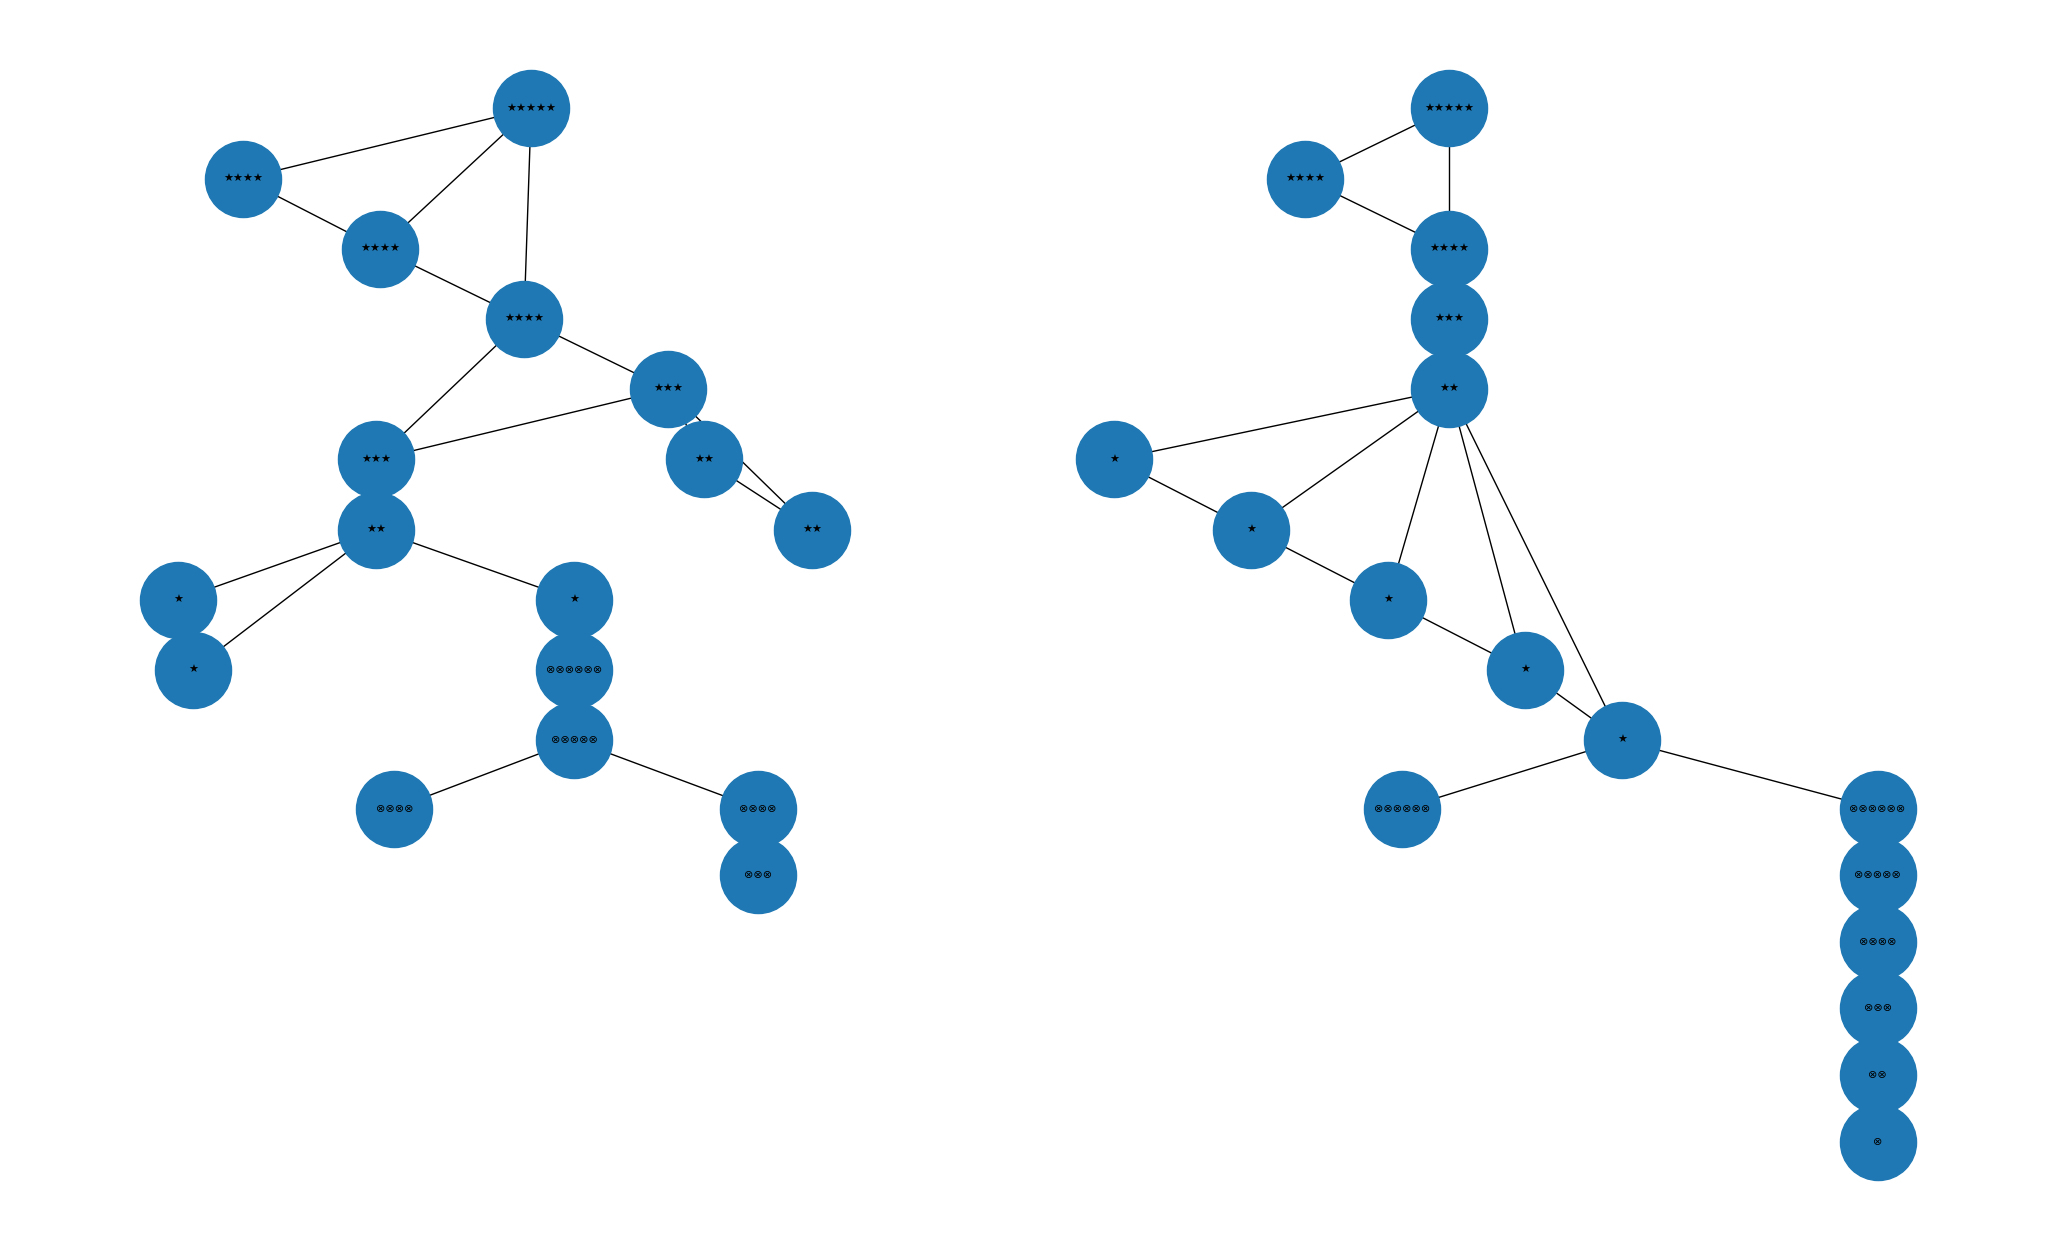
\includegraphics[scale=.3]{report1/img/documentation/test_structure_output.png}
    \caption{Example of the structure for input "ABBBCDDCDEE\#EFGH\#HIABBCDEEEEEF\#FGH\#I\#J\#K"}
    \label{fig:teststructureoutput}
\end{figure}

\begin{figure}
    \centering
    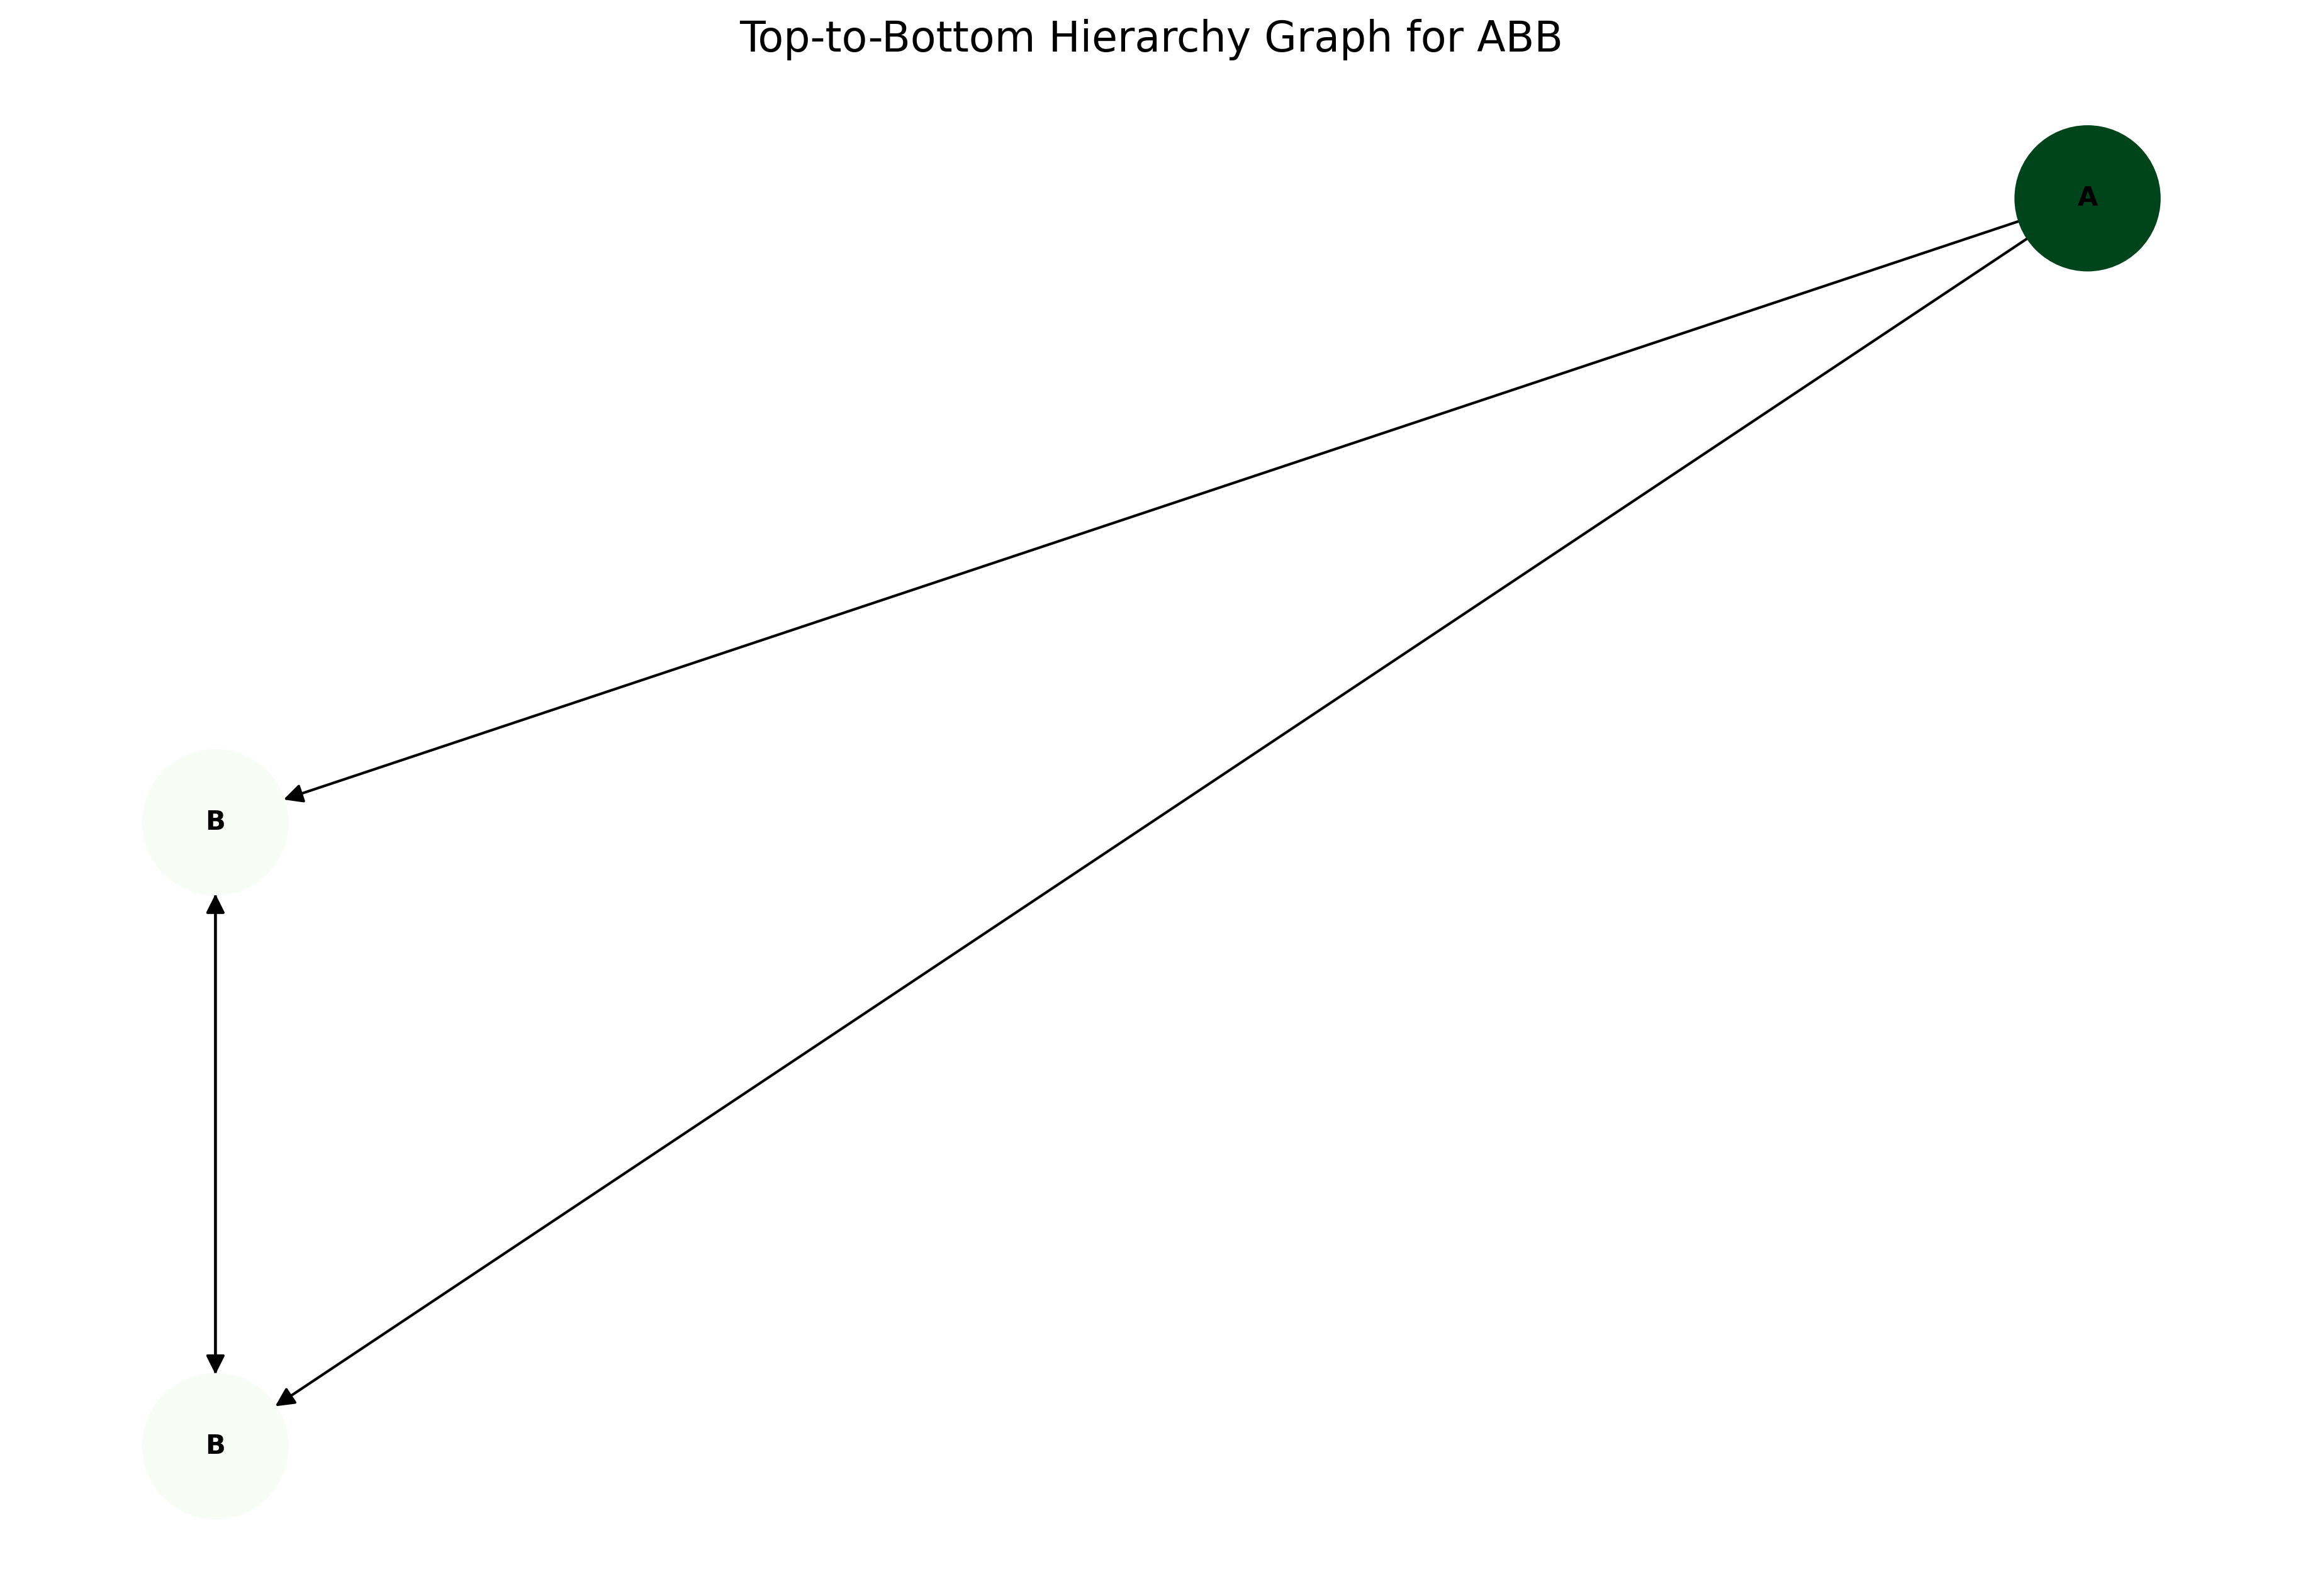
\includegraphics[scale=.5]{report1/img/documentation/ABB.png}
    \caption{Example of the structure for input "AB\#B"}
    \label{fig:abb}
\end{figure}
\pagebreak 
